\subsection{\ainterface}
\label{sec:admininterface}
The \admin[] interface is illustrated in figure \ref{fig:admin_interface}.
After login, the \admin[] is presented with the \textit{main} window. All the window have a back function which enables the \admin[] to return to the previous window.


\begin{figure}[p]
	\centering
		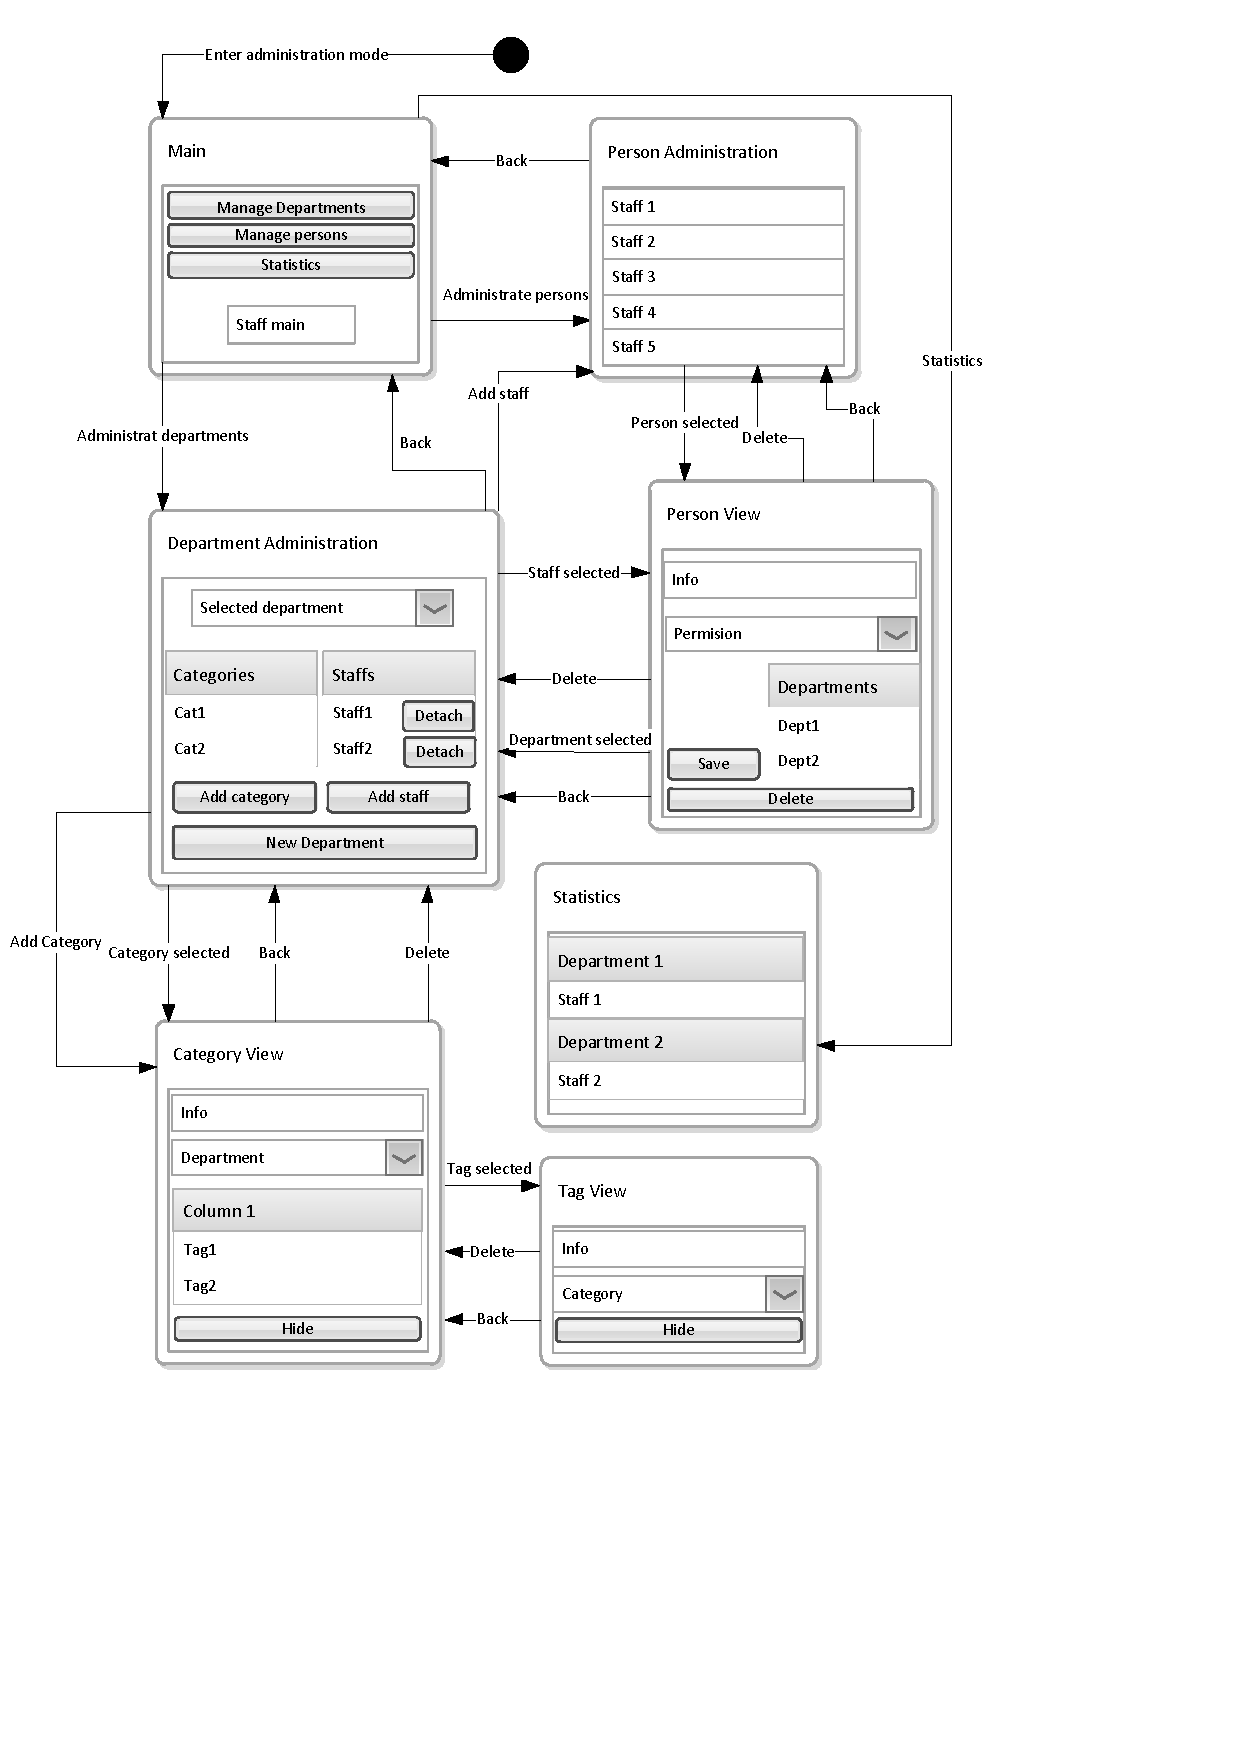
\includegraphics[width = \textwidth, clip=true, trim=0 4cm 5cm 0]{input/application_domain_analysis/Navigation_DiagramAdmin.pdf}
	\morscaption{The navigation diagram of the admin interface}
	\label{fig:admin_interface} %fig:Navigation_DiagramAdmin
\end{figure}

\subsubsection{Main}
The ``Main'' \admin[] window gives access to administration options and the functionality from the \astaff[] and \aclient[] main windows. The window contains: 
\begin{itemize}
	\item The button ``Manage Departments'' directs the \admin[] to the ``Department Administration'' window.  
	\item The button ``Manage People'' directs the \admin[] to the ``Person Administration'' window.
	\item The button ``statistics'' directs the \admin[] to the ``statistics'' window.
\end{itemize}
The window includes the buttons from the \astaff[] and \aclient[] ``main'' window.
%The ``Main'' administrator window contains two new  and ``Administrate persons''. The buttons from the ``Main'' \astaff and \aclient window are also shown.  

\subsubsection{Person Administration}
When the ``person Administrate'' window is opened, the \admin[] is able to browse through all \astaff[] members. The window contain the following element:
\begin{itemize}
	\item A list with all the persons in the application.
\end{itemize}

\subsubsection{Department Administration}
This window shows a list of staff and categories for the selected department.
The ``Department administration'' contains the following:
\begin{itemize}
	\item A dropdown menu where department can be selected.
	\item A list of \astaff[] members who are a part of the selected department.
	\item A list of categories which is related to the department.
\end{itemize}
When the \astaff[] is clicked the \admin[] is send to the ``person view''.
When a category is clicked the \admin[] is send to the ``Category view''. 


\subsubsection{Person View}
The ``person view'' shows information about a selected person.
The window contains the following elements:
\begin{itemize}
	\item A info field where relevant information is displayed about the person
	\item A dropdown where roles can be set.
	\item A dropdown where departments can be set.
	\item The button ``delete'' which deletes the person and sends the user back to the previous window. 
\end{itemize}

\subsubsection{Category View}
The ``Category View'' window shows information about the selected category and allows it to be modified. The window contains the following: 

\begin{itemize}
	\item An info field where relevant information is displayed.
	\item A list with all the tags belonging to the category.
	\item The ``Create new tag'' which send the \admin[] to ``Tag View'' window.
	\item The ``hide'' button which hide category and its tags. 
\end{itemize}
Each tag have an ``edit'' button which allows a tag to be modified, the button sends the \admin[] to the ``Tag view'' window. 

\subsubsection{Tag View}
This window is used to create new tags and edit already existing tags.
It contains the following:
\begin{itemize}
	\item A info field which can be edited.
	\item An ``Hide'' button which hide the tag.
	\item An ``save'' button which save the changes made.
\end{itemize}
When the hidden button is pressed then the \admin[] is directed back to the ``category view'' window.

